\documentclass[dvipsnames,tikz]{standalone}
\usepackage{amsmath}
\usepackage{xcolor}
\usepackage{tikz}
\usepackage{cmbright}      % sansfont
\usetikzlibrary{calc}
\usetikzlibrary{decorations.pathreplacing,calligraphy,3d}



\begin{document}
	% add color=white for dark mode
	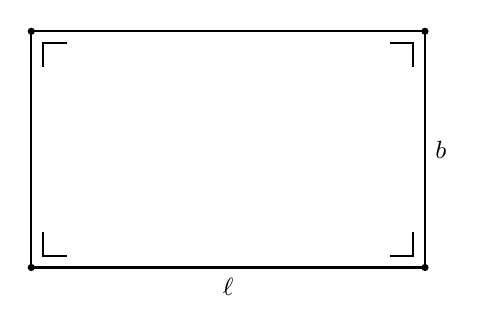
\begin{tikzpicture}[thick, color=black] 
		\draw (0,0) rectangle (5,3);
		\draw[shift={(0.15,0.15)}] (0.3,0) -- (0,0) -- (0,0.3);
		
		\begin{scope}[shift={(5,0)}, rotate=90]
			\draw[shift={(0.15,0.15)}] (0.3,0) -- (0,0) -- (0,0.3);
		\end{scope}
	
		\begin{scope}[shift={(5,3)}, rotate=180]
			\draw[shift={(0.15,0.15)}] (0.3,0) -- (0,0) -- (0,0.3);
		\end{scope}
		
		\begin{scope}[shift={(0,3)}, rotate=-90]
			\draw[shift={(0.15,0.15)}] (0.3,0) -- (0,0) -- (0,0.3);
		\end{scope}
		
		\begin{scope}[font=\small]
			\fill (0,0) circle (1.3pt);
			\fill (5,0) circle (1.3pt);
			\fill (5,3) circle (1.3pt);
			\fill (0,3) circle (1.3pt);
			\draw (2.5,0) node [below] {$\ell$};
			\draw (5,1.5) node [right] {$b$};
		\end{scope}
	\end{tikzpicture} 
	
\end{document}